\documentclass[a4paper]{article}
\usepackage{epsfig}
\usepackage{german}

\title{BSEvolution}
\author{Ingo Ruhnke grumbel@gmx.de}

\begin{document}
\maketitle

\tableofcontents

\section{Was ist BSEvolution?}

BSEvolution ist ein einfaches GUI gesteuertes Programm zur Simulation
der Evolution zweier hypothetischer Lebewesen, n"amlich des
Biegosaurus und der Stachelophyte.

\subsection{Hard- und Software Anforderungen}
BSEvolution setzt auf Java auf, es sollte mit allen JDK 1.2 f"ahigen
Umgebungen "ubersetzen und laufen lassen. Getestet wurde es aber nur
mit Sun's Java 1.2 und 1.3.

An Hardware empfiehlt sich ein Pentium 133 oder vergleichbares. 8bit
sind mindestens f"ur die Grafikdarstellung notwendig, f"ur optimale
Grafikdarstellung sollte die Grafikkarte aber in der Lage sein 16bit
darzustellen.

\section{Die Evolution}
\subsection{Der Biegosaurus und die Stachelophyte}

Der Biegosaurus ist pflanzenfressender Dinosaurier mit einem langem,
aber unbeweglichen, um 90 Grad abgewinkelten Hals.  Seine bevorzugte
Pflanze ist die Stachelophyte. Seine existens wird durch lediglich
zwei Gene bestimmt, eines ist f"ur die H"ohe des Halses, das andere
f"ur die Breite.
 
Die Stachelophyte ist eine hohe, palmenartige Pflanze mit
wohlschmeckende gr"une Blattern.  Zum Schutz vor Fressfeinden hat sie
am Boden lange giftige Stacheln entwickelt. Auch die Stachelophyte
besitzt nur zwei Gene, eines ist f"ur die H"ohe des Stammes zu
st"andig, das andere f"ur die L"ange der Stacheln.


\subsection{Wie geschieht die Evolution?}

Die Evolution geschieht wie "ublich zuf"allig. Pro Evolutions Schritt
werden jeweils zwei neue Lebewesen erzeugt, die um je eine H"ohen oder
Breiten Einheit von dem Ursprungstier abweichen k"onnen. Es "uberlebt
dann der Biegosaurus der am n"achsten an der gr"unen Bl"attern der
Stachelophyte dran ist, bzw. die Stachelophyte die am meisten vom
Biegosaurus entfernt ist. Wenn die Gesamtl"ange, also Breite plus
H"ohe, einen festgelegten Wert "uberschreitet wird noch ein
,,Strafwert'' auf den Abstand addiert, so das die Lebewesen nicht
"uber diesen hinauswachsen.


\section{Die Simulation}

BSEvolution bietet die M"oglichkeit die beschriebene Evolution zu
simulieren und zu visualisieren, Abbildung \ref{bsgui} zeigt
Interface in Aktion.

\begin{figure}[h]
\centerline{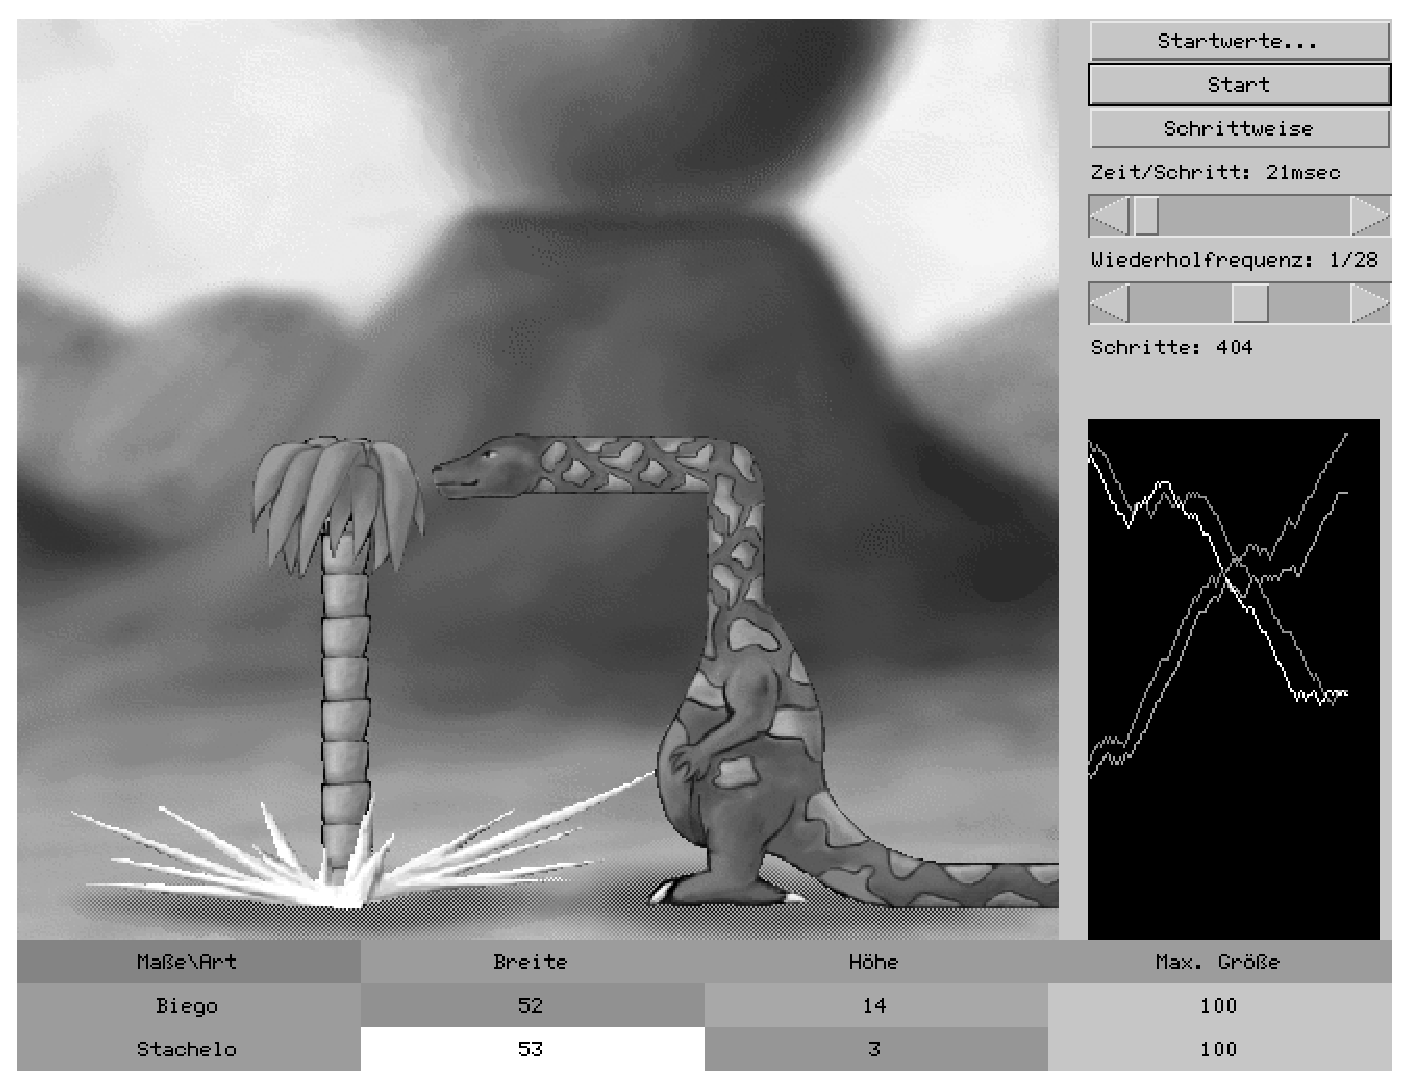
\includegraphics[height=75mm]{bsevolution_gui.ps}}
\caption{Tblaeua}
\label{bsgui}
\end{figure}

"Uber den Knopf \emph{Startwerte...} lassen sich die Anfangsbedingunen
f"ur die Evolution setzen, dieses Umfasst die H"ohe und Breite der
Lebewesen, sowie die Maximalen Gr"o"se, bei deren "ubertretung der
interne Strafwert greift.

Die Evolution selbst l"a"st sich "uber den Start Knopf anwerfen, dabei
wird die Evolution solange fortgef"uhrt bis sie "uber selbigen Knopf,
seine Beschriftung "andert sich zu \emph{Stop}, beendet wird.

Der Knopf \emph{Schrittweise} f"uhrt dazu das ein Evolutionsschritt
durchgef"uhrt wird und danach sofort wieder gestoppt wird. Wird der
Knopf bei einer laufenden Evolution gedr"uckt wird diese unterbrochen.

Der Schieberegler \emph{Zeit/Schritt} gibt die Zeit an die pro
Evolutionsschritt zwischen den Evolutionsschritten gewartet wird.
Kleinere Werte ergeben eine schnellere Evolution.

Die \emph{Wiederholfrequenz} gibt an bei jedem wievielten durchlauf
die Grafik neugezeichnet wird. Speziell bei langsameren Systemen
empfielt es sich diesen Wert etwas h"oher zu setzen, damit die
Evolution schneller geht und ver"anderungen gut sichtbar sind.

Der Graph in der rechten Ecke zeigt den Verlauf der Evolution, er
zeigt die H"ohe und Breite der Lebewesen. Die X-Achse umfasst 145
Evolutionsschritte, die Y-Achse wird relative zur festgelegten
Maximalen Gr"o"se skaliert. Die Farben der Graphen sind identisch zu
denen in der untenliegenden Anzeige f"ur die aktuelle H"ohe und Breite
der Lebewesen.

Die gro"se Grafik links zeigt ebenso die aktuelle H"ohe und Breite der
Lebewesen in einer visuell Ansprechenden Form. 

\section{Beispiele}

\subsection{Evolution mit gut sichtbaren Ver"anderungen}

Damit man von der Evolution auch etwas zu sehen bekommt empfiehlt es
sich die Wiederholfrequenz "uber den Schieberegler niedrig zu setzen,
also zum Beispiel auf 1/10. Ebenso empfiehlt es sich die Zeit pro
Schritt Differenz sehr niedrig zu setzen, also zum Beispiel auf
100msec. Damit wird erreicht das etwa jede Sekunde ein neues Bild
gezeichnt wird.  "Uber den Knopf \emph{Startwerte...} kann man dann
noch die Startwerte nach belieben ver"andern, die
Standardeinstellungen sollten aber schon ganz gute Ergebnisse liefern.
Durch einen Druck auf \emph{Start} kann, wenn alles nach Wunsch
eingestellt ist die Evolution angesto"sen werden.

\subsection{Genaue Darstellung jedes Evolutions Schrittes}

Um jeden Evolutionsschritt zu sehen, empfiehlt es sich die
\emph{Wiederholfrequenz} auf 1/1 zu setzen, somit erreicht man das
jeder Schritt gezeigt wird. Damit aber auch langsame Rechner hinter
herkommen, muss noch die Zeit pro Schritt angepasst werden, 1000msec
ist hier ein guter Wert. Die Startwerte k"onnen wie schon geschrieben
nach belieben gesetzt werden.

\end{document}

%% EOF %%